Die Einrichtungszeit ist die Zeit, die benötigt wird, um die 
Zwei-Faktor-Authentisierung beim Webdienst einzurichten. Die Messung 
beginnt, sobald der Proband auf der Website die Anweisungen zur 
Einrichtung sieht (QR-Code scannen, initiales TOTP eingeben). Nach der 
Eingabe und Bestätigung des initialen TOTPs wird die Messung beendet.
\\\\
Bei den 11 Probanden wurde jeweils ein Wert für die Einrichtungszeit 
gemessen. Ein Boxplot sowie die Verteilung der Werte ist in Abb. \ref
{fig: studie setup time boxplot} bzw. Abb. \ref{fig: studie setup time dist} dargestellt. Auffällig ist, dass ungefähr die Hälfte der Einrichtungen nicht länger 
als ca. 200~s dauerte, während die verbleibenden Einrichtung länger als 
ca. 290~s dauerten. Durchschnittlich haben die Probanden dem Median 
zufolge 177~s und dem Mittelwert nach 228~s benötigt (siehe Anhang \ref
{anh: studie ergebnisse setup} Tab. \ref{tab: studie setup time}). Die Spannweite 
der Zeiten reicht von 84~s bis zu 348~s.
\newpage
\begin{figure}[h]
    \begin{minipage}[b]{.42\textwidth}
        \centering
        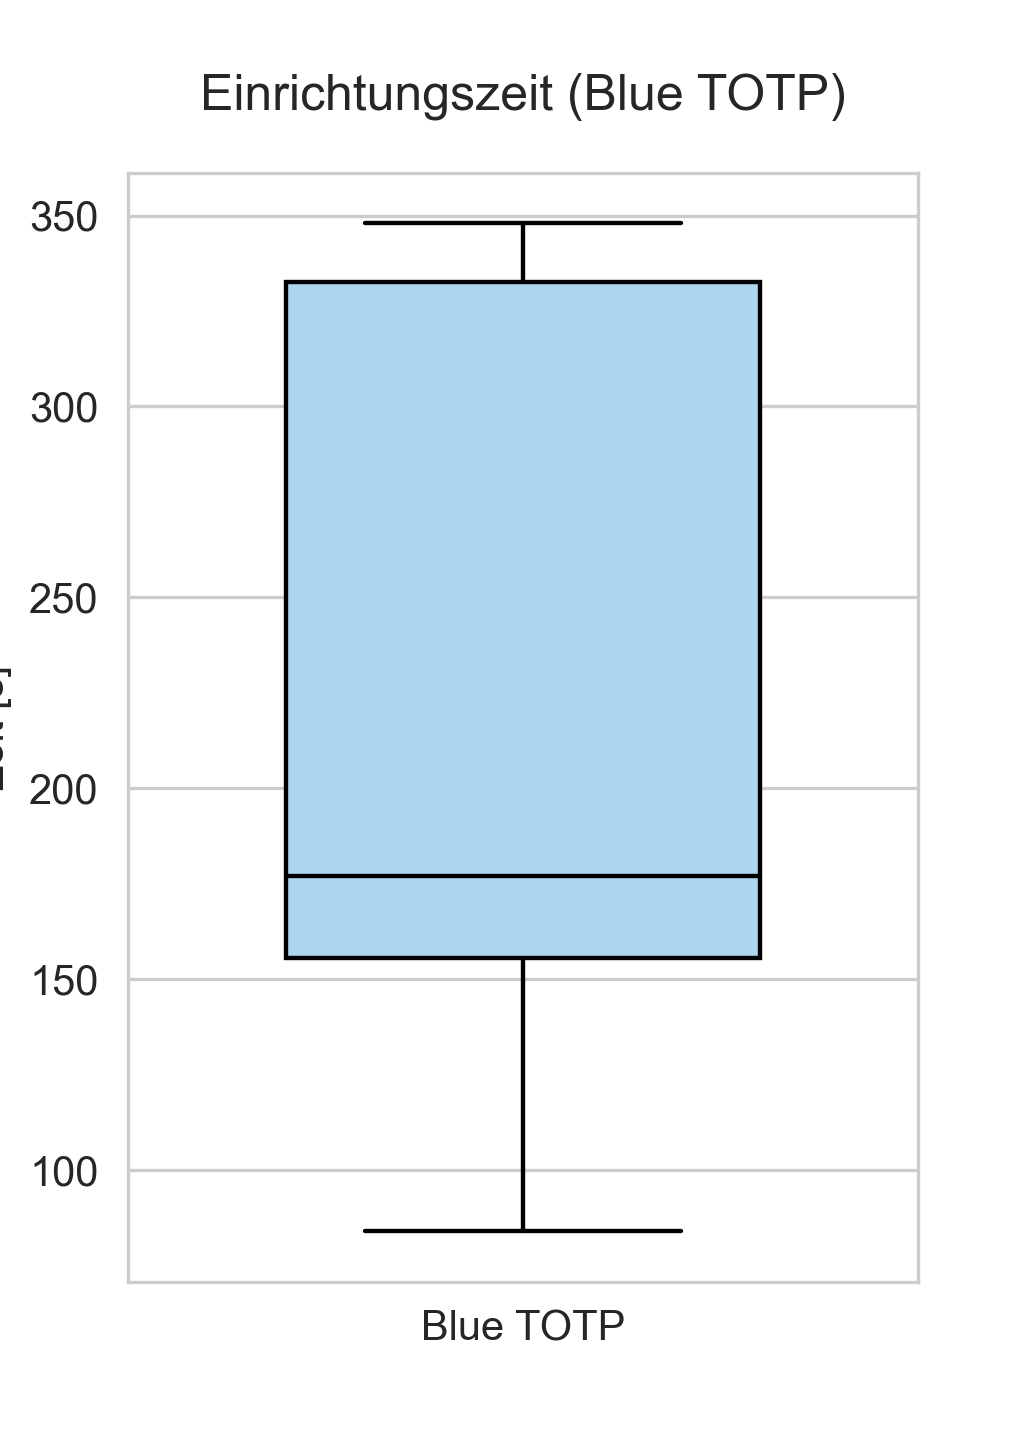
\includegraphics[width=0.8\linewidth]{data_processing/timings/results/setup_timings_boxplot.png}
        \caption[Einrichtungszeit von Blue TOTP]{Einrichtungszeit von Blue TOTP}
        \label{fig: studie setup time boxplot}
    \end{minipage}
    \hfill
    \begin{minipage}[b]{.54\textwidth}
        \centering
        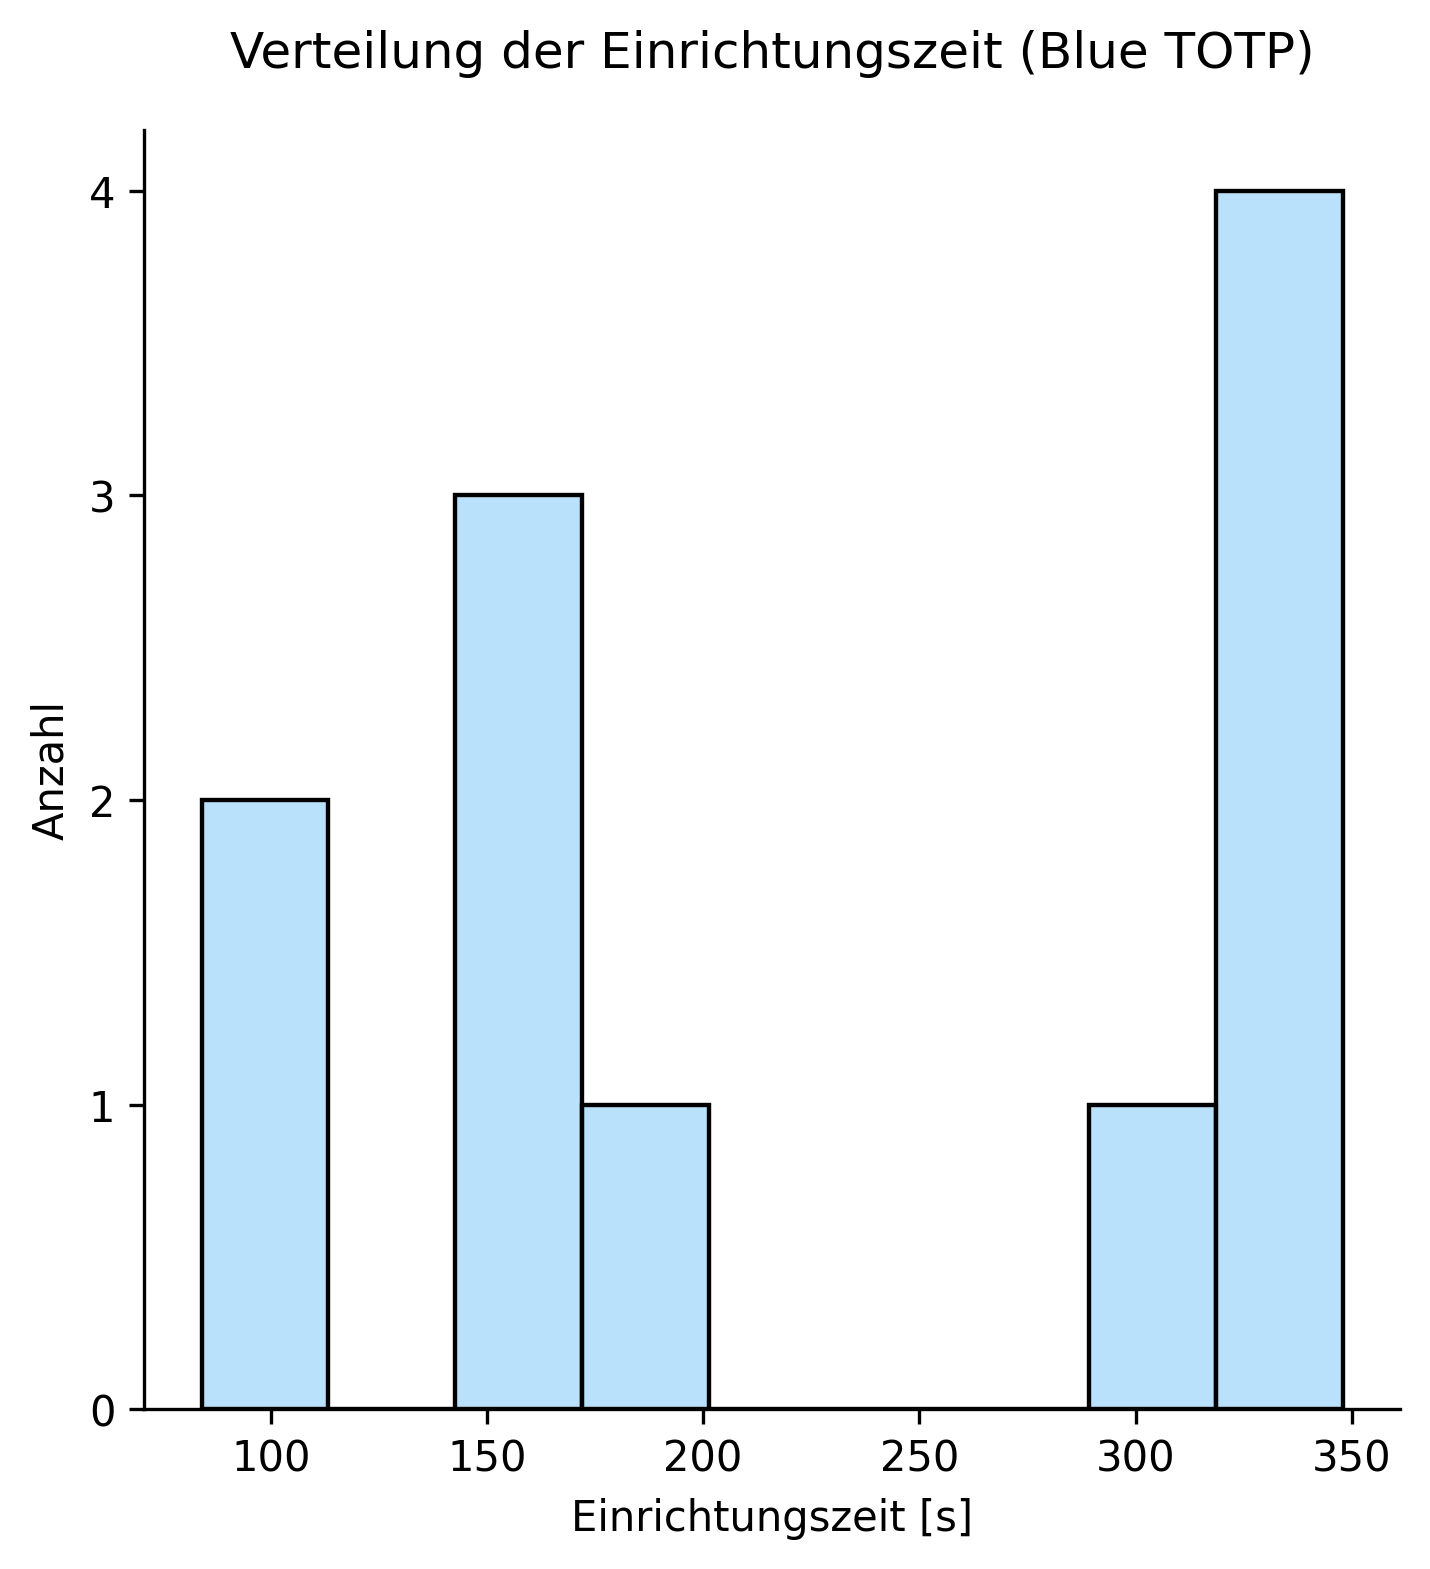
\includegraphics[width=0.78\linewidth]{data_processing/timings/results/distribution_of_setup_data.png}
        \caption[Verteilung der Einrichtungszeit von Blue TOTP]{Verteilung der Einrichtungszeit von Blue TOTP}
        \label{fig: studie setup time dist}
    \end{minipage}
\end{figure}
